\documentclass[aspectratio=169,12pt]{beamer}
\usepackage{eafitml}
\usepackage{colortbl}
\usepackage{qrcode}

% ---------------------------------------------------------------- local macros
\setbeamertemplate{section in toc}{\leavevmode{\color{mlgold}\inserttocsectionnumber.}~\inserttocsection\par}
\setbeamertemplate{subsection in toc}{\leavevmode\leftskip=2.2em\small\mdseries\inserttocsubsection\par}
\setbeamerfont{section in toc}{series=\bfseries,size=\normalsize}

% gold header + light teal body (e.g. "Casos extremos", "Objetivo")
\newtcolorbox{goldbox}[1][]{enhanced,sharp corners,boxrule=0pt,frame hidden,
  colback=mltealbg,colbacktitle=mlgold,coltitle=white,
  fonttitle=\bfseries\small,left=4pt,right=4pt,top=2pt,bottom=2pt,
  toptitle=1pt,bottomtitle=1pt,before skip=4pt,after skip=4pt,title={#1}}

% Plain frame with an image placed at a given bbox (pt, from top-left of the
% 453.5 x 255.1 pt page): \placedframe{file}{x0}{y0}{x1}
\newcommand{\placedframe}[4]{%
  \begin{frame}[plain]
    \begin{tikzpicture}[remember picture,overlay]
      \node[anchor=north west,inner sep=0pt] at ([xshift=#2pt,yshift=-#3pt]current page.north west)
        {\includegraphics[width=\dimexpr #4pt - #2pt\relax]{#1}};
    \end{tikzpicture}
  \end{frame}}

% keep beamer's compact list spacing inside \small / \footnotesize
\makeatletter
\let\ml@beamerlisti\@listi
\expandafter\apptocmd\csname small \endcsname{\let\@listi\ml@beamerlisti}{}{}
\expandafter\apptocmd\csname footnotesize \endcsname{\let\@listi\ml@beamerlisti}{}{}
\makeatother
\newcolumntype{L}[1]{>{\raggedright\arraybackslash}p{#1}}
\newcommand{\colhead}[1]{\textbf{#1}\par\vspace{2pt}}
\newcommand{\hrow}{\rowcolor{mlcream}}
\renewcommand{\arraystretch}{1.15}
\newcommand{\ind}{\mathbb{1}}
% placeholder for data the instructor must confirm (dates, room, links)
\newcommand{\pend}[1]{\textcolor{mlred}{\textbf{[#1]}}}
\usetikzlibrary{decorations.pathreplacing}
\lstset{numbers=left,numberstyle=\tiny\color{mlgray},numbersep=8pt,backgroundcolor={}}

\title[Evaluación, validación e hiperparámetros]{Evaluación moderna, validación e hiperparámetros}
\subtitle{Aprendizaje Automático · Parte 1}
\author[Aprendizaje Automático]{Andrés Vásquez Restrepo\\[2pt]{\normalfont\small\texttt{avasquezr3@eafit.edu.co}}}
\institute{SI7009 - 1 (5553)\\Universidad EAFIT}
\date{2026-2 -- Medellín}
\titlegraphic{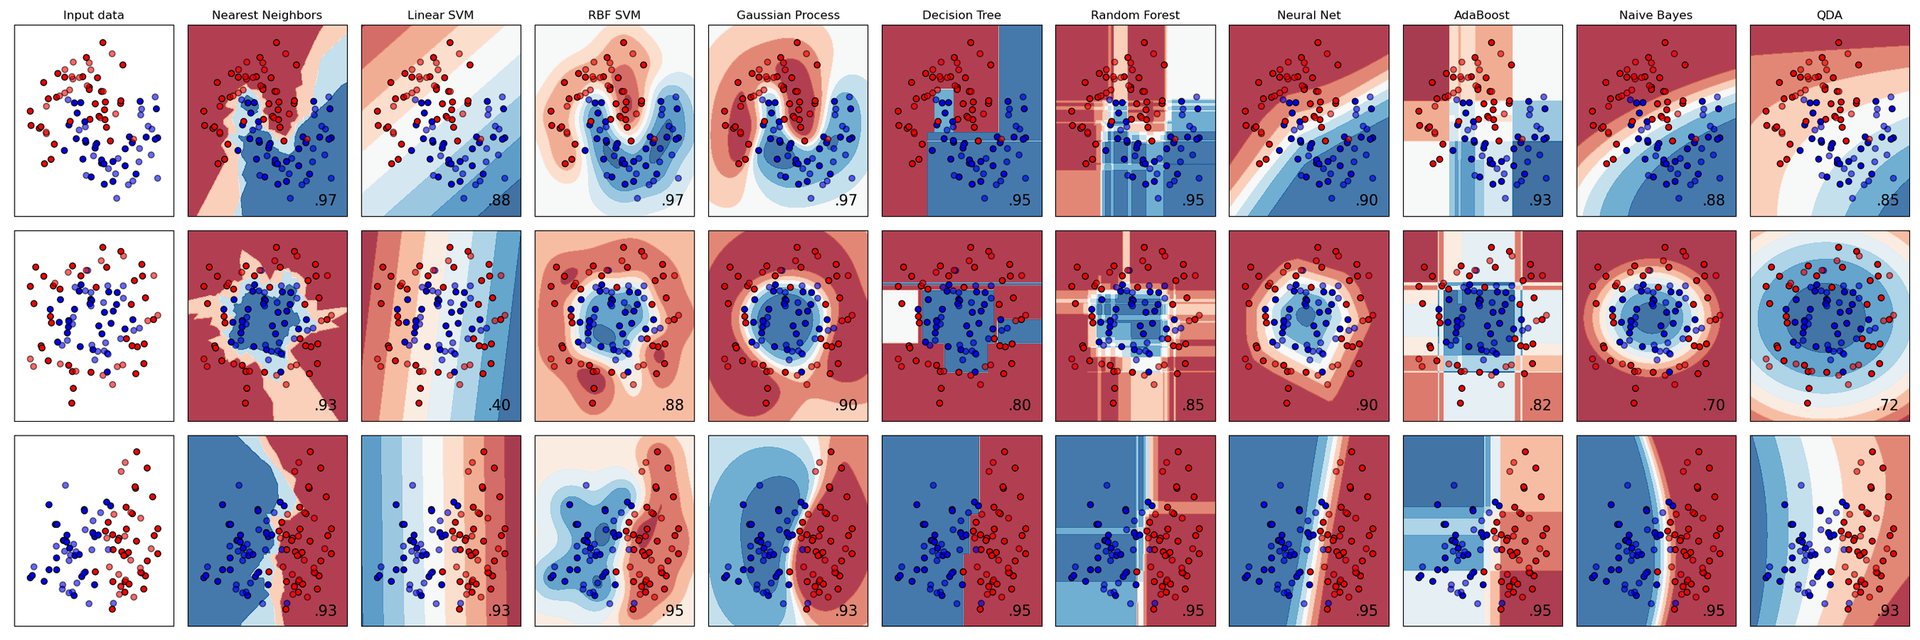
\includegraphics[width=5cm]{figures/img_p001_01.png}}

\begin{document}

% ============================================================ p1
\titleframe
\addtocounter{framenumber}{1}

% ============================================================ p2
\begin{frame}{Contenido}
  \setbeamertemplate{subsection in toc}{}\tableofcontents
\end{frame}

% ============================================================ p3-4
\section{Panorama del curso}
\sectionframe{Panorama del curso}

% ============================================================ p5
\begin{frame}{Aprendizaje Automático: visión del curso}
  \large
  \begin{defbox}[\Large Promesa del curso]
    Diseñar, evaluar, comparar e interpretar soluciones de Machine Learning con criterio defendible.
  \end{defbox}
  \begin{itemize}
    \item 6 sesiones presenciales intensivas (3 unidades)
    \item Bloque 17, Aula 303 \pend{confirmar aula 2026-2}
  \end{itemize}
\end{frame}

% ============================================================ p6
\begin{frame}{Cómo vamos a aprender}
  \begin{columns}[T]
    \begin{column}{0.31\textwidth}
      \begin{defbox}[\mbox{Presentaciones}]
        Narrativa conceptual, errores frecuentes, criterios de decisión.
      \end{defbox}
    \end{column}
    \begin{column}{0.31\textwidth}
      \begin{toolbox}[Notebooks]
        Demos reproducibles en Python con datasets reales.
      \end{toolbox}
    \end{column}
    \begin{column}{0.31\textwidth}
      \begin{taskbox}[Práctica]
        Decisiones técnicas aplicadas al taller, exposición y PI.
      \end{taskbox}
    \end{column}
  \end{columns}
  \vspace{6pt}
  \begin{rulebox}[Regla metodológica]
    El código que corre no basta: el experimento debe ser válido, comparable y defendible.
  \end{rulebox}
\end{frame}

% ============================================================ p7
\begin{frame}{Sistema de evaluación}
  \centering\footnotesize
  \begin{tabular}{@{}l r L{0.58\textwidth}@{}}
    \toprule
    \hrow \textbf{Componente} & Peso & Qué evalúa \\
    \midrule
    \textbf{Taller modular único} & 20\,\% & Formulación, validación cruzada, comparación, threshold y decisión final \\
    \textbf{Exposición avanzada} & 20\,\% & Comunicación técnica, ejemplo en Python y reproducibilidad \\
    \textbf{Examen final} & 25\,\% & Comprensión conceptual individual y juicio metodológico \\
    \textbf{Proyecto Integrador} & 35\,\% & Aporte analítico defendible dentro del PI \\
    \bottomrule
  \end{tabular}
  \vspace{6pt}
  \begin{keybox}[Criterio]
    \small La evaluación mide criterio técnico, no recitación de algoritmos.
  \end{keybox}
\end{frame}

% ============================================================ p8
\begin{frame}{Roadmap de sesiones}
  \centering\footnotesize
  \begin{tabular}{@{}c l L{0.5\textwidth} L{0.22\textwidth}@{}}
    \toprule
    \hrow \textbf{Sesión} & Unidad & Tema central & Dataset / artefacto \\
    \midrule
    \textbf{1} & U1 & Evaluación, métricas, CV, calibración y HPO; árboles, ensembles, boosting y Optuna & Fraude transaccional \\
    \textbf{2} & U1 & Teoría de boosting moderno: XGBoost, LightGBM, CatBoost y otros modelos & Fraude + Optuna \\
    \textbf{3} & U2 & ML para series de tiempo y walk-forward validation & Serie temporal \\
    \textbf{4} & U2 & Sistemas de recomendación e interpretabilidad (SHAP) & MovieLens \\
    \textbf{5} & U3 & Reducción de dimensión y clustering & Online Retail \\
    \textbf{6} & U3 & Mini-Batch K-Means, outliers, calibración y drift & Online Retail \\
    \bottomrule
  \end{tabular}
  \vspace{2pt}

  \scriptsize U1: supervisado moderno \quad U2: secuencia, tiempo y personalización \quad U3: estructura y confiabilidad
\end{frame}

% ============================================================ p9
\begin{frame}{Proyecto Integrador 1: qué es y qué exige}
  \begin{defbox}[Idea central]
    Proyecto transversal para resolver una problemática real con datos reales, integrando modelado, tecnología y comunicación.
  \end{defbox}
  \begin{itemize}
    \item Vale 35\,\% de cada materia
    \item Debe seguir una metodología explícita: problema, datos, preparación, modelado, evaluación y despliegue
    \item Cada equipo debe definir temprano: problema, fuentes de datos, restricciones y ruta de solución
  \end{itemize}
  \begin{keybox}[Aporte por curso]
    AA: baseline, modelos, validación e interpretación\\
    Big Data: arquitectura, pipeline y despliegue\\
    Visualización: app/dashboard, pitch y defensa
  \end{keybox}
\end{frame}

% ============================================================ p10
\begin{frame}{Qué se evalúa y qué deben entregar}
  \begin{columns}[T]
    \begin{column}{0.47\textwidth}
      \begin{taskbox}[Entregables finales]
        \begin{itemize}
          \item Documento consolidado
          \item Presentación final
          \item GitHub reproducible
          \item Sustentación: 20 min máx.
        \end{itemize}
      \end{taskbox}
    \end{column}
    \begin{column}{0.47\textwidth}
      \begin{toolbox}[Rúbrica mínima en AA]
        \begin{itemize}
          \item problema, tipo de target y métrica claros
          \item baseline explícito
          \item validación cruzada correcta
          \item modelos pertinentes
          \item análisis de resultados
        \end{itemize}
      \end{toolbox}
    \end{column}
  \end{columns}
  \begin{rulebox}[Hitos]
    Preliminar: \pend{DD/MM} \quad Propuesta: \pend{DD/MM} \quad Entrega final maestría: \pend{DD/MM}\\
    Sustentación: \pend{DD/MM}
  \end{rulebox}
\end{frame}

% ============================================================ p11
\begin{frame}{Exposiciones: mini-system}
  \footnotesize
  \begin{defbox}[Rol en el curso]
    Componente formal del curso que vale 20\,\%. No reemplaza la clase: amplía el horizonte con temas modernos no cubiertos de forma central en las cinco sesiones.
  \end{defbox}
  \begin{columns}[T]
    \begin{column}{0.47\textwidth}
      \begin{taskbox}[Política operativa]\scriptsize
        \begin{itemize}
          \item Asignación por orden de escogencia
          \item Individual o en pareja
          \item Tríos solo si la matrícula lo exige
          \item Un tema no se repite hasta agotar el banco
          \item Cierre de escogencia: \textbf{fin de la Sesión 2}
        \end{itemize}
      \end{taskbox}
    \end{column}
    \begin{column}{0.47\textwidth}
      \begin{toolbox}[Entrega mínima]\scriptsize
        \begin{itemize}
          \item PDF
          \item GitHub público reproducible
          \item Ejemplo computacional reproducible
          \item 20 min de exposición + 5 min de preguntas
          \item Participación equilibrada
        \end{itemize}
      \end{toolbox}
    \end{column}
  \end{columns}
  \begin{rulebox}[Calendario de exposiciones]
    \footnotesize Temas definidos a más tardar al \textbf{final de la Sesión 2}. Las exposiciones inician en la \textbf{Sesión 3}; el número de exposiciones por sesión se define según la cantidad de grupos.
  \end{rulebox}
\end{frame}

% ============================================================ p12
\begin{frame}{Banco de temas oficial}
  \begin{tikzpicture}[remember picture,overlay]
    \node[anchor=north east,inner sep=2pt,fill=white] at ([xshift=-10pt,yshift=-4pt]current page.north east)
      {\href{https://eafit-my.sharepoint.com/:x:/g/personal/avasquezr3_eafit_edu_co/IQBMNr9rRCRzSIhl0wmT5yroAXJ4WnD7ZvdjMnQujZHcw5Y?e=CsqvSX}{\qrcode[height=1.25cm]{https://eafit-my.sharepoint.com/:x:/g/personal/avasquezr3_eafit_edu_co/IQBMNr9rRCRzSIhl0wmT5yroAXJ4WnD7ZvdjMnQujZHcw5Y?e=CsqvSX}}};
  \end{tikzpicture}%
  \centering\footnotesize
  \begin{tabular}{@{}l L{0.78\textwidth}@{}}
    \toprule
    \hrow \textbf{Línea} & Temas disponibles \hfill \textbf{Inscripción:} \href{https://eafit-my.sharepoint.com/:x:/g/personal/avasquezr3_eafit_edu_co/IQBMNr9rRCRzSIhl0wmT5yroAXJ4WnD7ZvdjMnQujZHcw5Y?e=CsqvSX}{\textcolor{eafitneon}{\underline{abrir hoja compartida}}} \\
    \midrule
    \textbf{Base} & Sistemas de recomendación avanzados; aprendizaje por refuerzo; aprendizaje semi-supervisado; aprendizaje federado; MLOps / deployment; restricciones en modelos; Explainable AI \\
    \midrule
    \textbf{Expansión} & Graph Neural Networks; Learning to Rank; uplift modeling y causal ML; active learning; continual learning; time-series transformers; tabular deep learning; AutoML y meta-learning \\
    \midrule
    \textbf{Avanzados} & Synthetic data; privacy-preserving ML; fairness; anomaly detection at scale; survival analysis; multi-objective optimization; weak supervision; foundation models tabulares o temporales \\
    \midrule
    \textbf{Sistemas} & Retrieval-augmented ML systems; ML para grafos dinámicos; bandits contextualizados; conformal prediction; uncertainty quantification; TinyML / energy efficient ML \\
    \bottomrule
  \end{tabular}
\end{frame}

% ============================================================ p13
\begin{frame}{Logística clave de arranque}
  \begin{block}{{\large Fechas docentes}}
    \pend{6 fechas docentes del semestre 2026-2}
  \end{block}
  \begin{alertblock}{{\large Importante}}
    \begin{itemize}
      \item Aula: Bloque 17, Aula 303 \pend{confirmar}.
      \item \pend{Festivos, clases re-localizadas o virtuales del semestre}.
      \item Sustentación institucional del PI: \pend{DD/MM}; no es clase regular.
    \end{itemize}
  \end{alertblock}
\end{frame}

% ============================================================ p14
\begin{frame}{Logística clave de arranque}
  \begin{taskbox}[\Large Desde la segunda semana]
    \footnotesize Tema y dataset del taller: \pend{definir}. Taller necesario para justificar:
    \large
    \begin{itemize}
      \item target y baseline;
      \item métrica y esquema de validación cruzada;
      \item threshold, costo y error dominante;
      \item conexión con el PI.
    \end{itemize}
  \end{taskbox}
\end{frame}

% ============================================================ p15
{\setbeamertemplate{background}{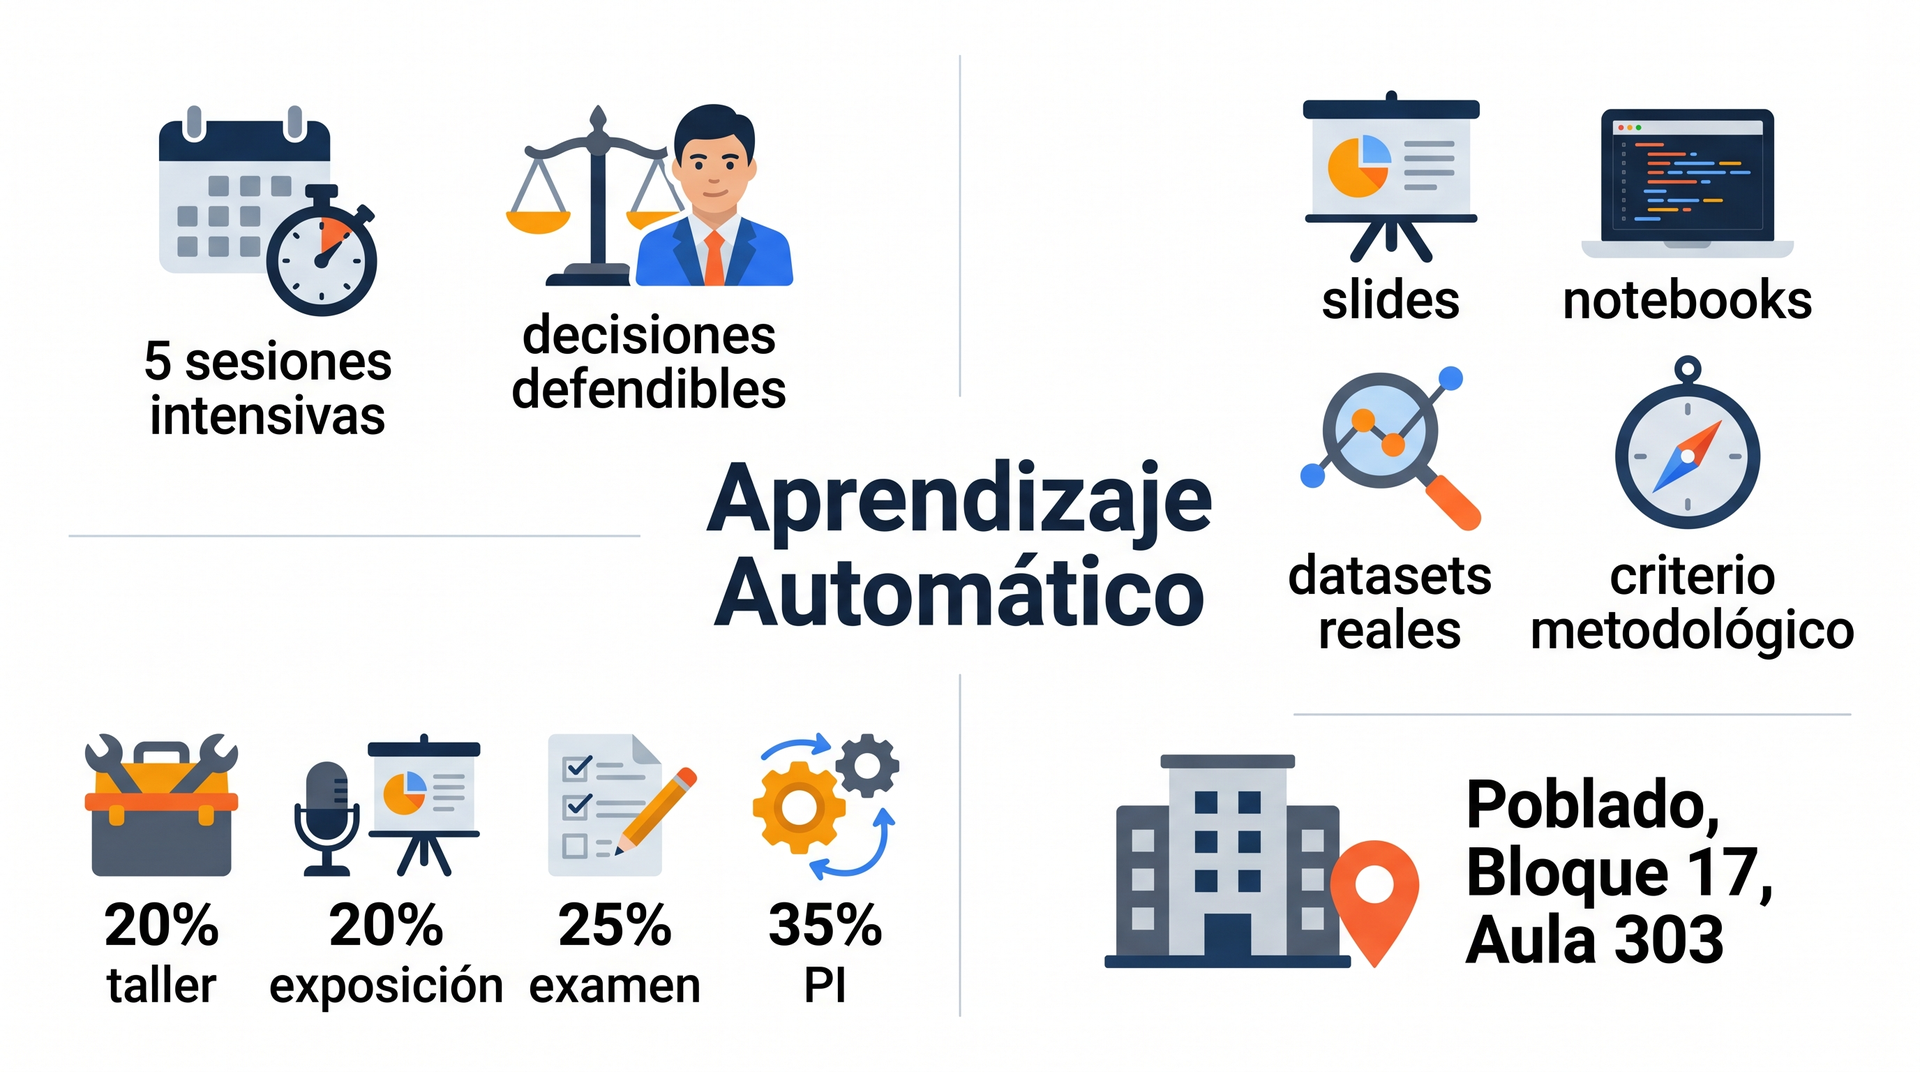
\includegraphics[width=\paperwidth,height=\paperheight]{figures/img_p015_03.png}}%
 \begin{frame}[plain]
   \begin{tikzpicture}[remember picture,overlay]
     \fill[white] ([xshift=31pt,yshift=-78pt]current page.north west) rectangle ([xshift=96pt,yshift=-106pt]current page.north west);
     \node[align=center,inner sep=0pt,font=\fontsize{11.5}{11.5}\selectfont\sffamily\bfseries] at ([xshift=63.5pt,yshift=-92pt]current page.north west) {6 sesiones\\intensivas};
   \end{tikzpicture}
 \end{frame}}

% ============================================================ p16
\begin{frame}{Ruta del curso: 6 sesiones, 3 unidades}
  \centering
  \begin{tikzpicture}[x=2.3cm,y=1cm]
    \draw[line width=3pt,mlteal] (0,0) -- (5,0);
    \foreach \i/\t/\d in {0/{evaluación, HPO,\\árboles y boosting}/fraude,
                          1/{teoría de\\boosting moderno}/XGBoost,
                          2/{series de\\tiempo}/walk-forward,
                          3/{recomendadores\\y SHAP}/MovieLens,
                          4/{reducción de dim.\\y clustering}/Online Retail,
                          5/{outliers,\\calibración y drift}/Online Retail}{
      \pgfmathtruncatemacro{\s}{\i+1}
      \node[circle,fill=mlgold,minimum size=11pt,inner sep=0pt] at (\i,0) {};
      \node[fill=mlbg,text=white,rounded corners=6pt,font=\footnotesize\bfseries,inner sep=4pt] at (\i,1.9) {Sesión \s};
      \node[align=center,font=\scriptsize\bfseries,text width=2.1cm] at (\i,0.9) {\t};
      \node[font=\scriptsize,text=mlgray] at (\i,-0.55) {\d};
    }
    \foreach \a/\b/\u in {-0.45/1.45/{U1 · Supervisado moderno},
                          1.55/3.45/{U2 · Secuencia, tiempo\\ y personalización},
                          3.55/5.45/{U3 · Estructura\\ y confiabilidad}}{
      \draw[decorate,decoration={brace,mirror,amplitude=5pt},mlgray] (\a,-0.95) -- (\b,-0.95)
        node[midway,below=6pt,font=\scriptsize\bfseries,text=mltitle,text width=4.4cm,align=center]{\hyphenpenalty=10000\exhyphenpenalty=10000 \u};
    }
  \end{tikzpicture}
\end{frame}

% ============================================================ p17
\section{Evaluación moderna y criterio}
\sectionframe{Evaluación moderna y criterio}

% ============================================================ p18
\begin{frame}{Un modelo puede verse bien y aun así fallar}
  \large
  \begin{center}
    En \textbf{Machine Learning} aplicado, un \emph{score} alto no prueba que el sistema sea útil.
  \end{center}
  Primero hay que preguntar qué problema se formuló, contra qué \emph{baseline} se comparó, qué métrica se usó y qué decisión se tomó.
  \vspace{8pt}
  \begin{itemize}
    \item Un modelo merece confianza solo cuando \emph{baseline}, métrica, validación cruzada, \emph{threshold}, calibración y costo del error forman un argumento defendible.
  \end{itemize}
\end{frame}

% ============================================================ p19
\begin{frame}{La provocación de hoy}
  \begin{center}
    \large Un sistema puede acertar en el $99{,}8$\,\% de las transacciones\\[4pt]
    y no detectar ningún fraude.
  \end{center}
  \vspace{4pt}
  \begin{columns}[T]
    \begin{column}{0.45\textwidth}
      \colhead{La cifra puede sonar excelente}
      \begin{itemize}
        \item muchos casos negativos;
        \item pocos eventos positivos;
        \item promedio global dominante.
      \end{itemize}
    \end{column}
    \begin{column}{0.45\textwidth}
      \colhead{La decisión puede ser inútil}
      \begin{itemize}
        \item no encuentra ninguno de los fraudes reales;
        \item falsos negativos costosos;
        \item ninguna alerta útil;
        \item falsa sensación de desempeño.
      \end{itemize}
    \end{column}
  \end{columns}
\end{frame}

% ============================================================ p20
\imageframe{figures/img_p020_05.png}

% ============================================================ p21
\begin{frame}{Qué vamos a aprender a defender}
  \centering\footnotesize
  \begin{tabular}{@{}l L{0.7\textwidth}@{}}
    \toprule
    \hrow \textbf{Decisión} & Pregunta que debe poder responder \\
    \midrule
    \textbf{Target} & ¿Qué variable queremos predecir y de qué tipo es? (hoy: binaria) \\
    \textbf{Baseline} & ¿Contra qué referencia se demuestra mejora? \\
    \textbf{Métrica} & ¿Qué error importa más en este problema? \\
    \textbf{Validación} & ¿Qué esquema de validación cruzada protege la generalización? \\
    \textbf{Threshold} & ¿Qué punto convierte score en acción? \\
    \textbf{Calibración} & ¿Las probabilidades significan lo que dicen? \\
    \textbf{Estrategia de desbalance} & ¿Qué intervención se valida sin contaminar el experimento? \\
    \bottomrule
  \end{tabular}
  \vspace{4pt}

  Al final de la sesión, cada resultado debe poder defenderse con una frase técnica, no con una impresión.
\end{frame}

% ============================================================ p22
\begin{frame}{El caso guía: fraude transaccional}
  \begin{columns}[T]
    \begin{column}{0.47\textwidth}
      \colhead{Problema}
      \begin{itemize}
        \item Clasificación binaria.
        \item Clase positiva rara.
        \item Evento positivo: transacción fraudulenta.
        \item Salida deseada: priorizar revisión o activar alerta.
      \end{itemize}
    \end{column}
    \begin{column}{0.47\textwidth}
      \colhead{Tensión operativa}
      \begin{itemize}
        \item Dejar pasar fraude puede ser costoso.
        \item Demasiadas alertas saturan revisión humana.
        \item Accuracy puede ocultar el fracaso.
        \item El threshold define la acción final.
      \end{itemize}
    \end{column}
  \end{columns}
  \vspace{6pt}
  El \emph{dataset} no se usará para ``correr modelos'', sino para aprender a evaluar decisiones.
\end{frame}

% ============================================================ p23
\placedframe{figures/img_p023_06.png}{38}{20}{413}

% ============================================================ p24
\begin{frame}{El mapa de la sesión}
  \small
  \begin{enumerate}
    \item Recordatorio: EDA, outliers y encoding.
    \item Métricas, costos y threshold.
    \item Workflow y baseline serio.
    \item Validación cruzada: estratificada, agrupada y temporal.
    \item ROC, PR y calibración.
    \item Optimización de hiperparámetros: grid, random, halving y nested CV.
  \end{enumerate}
  {\color{mlgray}\footnotesize Parte 2: árboles y bias--variance, ensembles, boosting moderno, balanceo y optimización bayesiana con Optuna.}
  \vspace{8pt}
  \begin{center}
    \Large\textbf{La historia completa es una cadena:} problema $\rightarrow$ datos $\rightarrow$ CV $\rightarrow$ métrica $\rightarrow$ threshold $\rightarrow$ decisión.
  \end{center}
\end{frame}

% ============================================================ R0 (nuevo)
\section{Recordatorio: datos antes de modelar}
\sectionframe{Recordatorio:\\datos antes de modelar}

% ============================================================ E1 (nuevo)
\begin{frame}{Recordatorio: EDA antes de modelar}
  {\color{mlgray}\footnotesize Viene del pre-curso. Aquí solo lo que condiciona la evaluación.}
  \begin{columns}[T]
    \begin{column}{0.47\textwidth}
      \colhead{Checklist mínimo}
      \begin{itemize}
        \item \texttt{df.info()}, \texttt{df.describe()}: tipos y rangos;
        \item nulos y duplicados;
        \item cardinalidad de categóricas;
        \item \textbf{balance del target}:\\ \texttt{y.value\_counts(normalize=True)}.
      \end{itemize}
    \end{column}
    \begin{column}{0.47\textwidth}
      \colhead{Tipo de target $\rightarrow$ tipo de problema}
      \footnotesize
      \begin{tabularx}{\linewidth}{@{}l >{\raggedright\arraybackslash}X@{}}
        \toprule
        \hrow Target & Problema \\
        \midrule
        Numérico continuo & Regresión \\
        Binario & Clasificación binaria \textbf{(hoy)} \\
        Categórico múltiple & Multiclase \\
        \bottomrule
      \end{tabularx}
    \end{column}
  \end{columns}
  \vspace{6pt}
  \begin{keybox}[Para esta sesión]
    El target es binario y muy desbalanceado: eso define métricas, validación y threshold.
  \end{keybox}
\end{frame}

% ============================================================ E2 (nuevo)
\begin{frame}{Recordatorio: outliers y limpieza}
  \begin{columns}[T]
    \begin{column}{0.47\textwidth}
      \colhead{Regla de los $3\sigma$}
      \[ |x_i - \mu| > 3\sigma \]
      \small Supone distribución aproximadamente normal; media y $\sigma$ son sensibles a los propios outliers.
    \end{column}
    \begin{column}{0.47\textwidth}
      \colhead{Rango intercuartílico (IQR)}
      \[ x_i \notin [\,Q_1 - 1{,}5\,IQR,\; Q_3 + 1{,}5\,IQR\,] \]
      \small Robusta: no depende de la normalidad.
    \end{column}
  \end{columns}
  \vspace{4pt}
  \small Limpieza: eliminar duplicados; imputar nulos (mediana, moda) \textbf{ajustando solo en train}.
  \begin{rulebox}[En fraude]
    El outlier puede ser justamente la señal: no se elimina sin analizarlo. La detección de anomalías (Isolation Forest, LOF) se retoma en la sesión de confiabilidad.
  \end{rulebox}
\end{frame}

% ============================================================ E3 (nuevo)
\begin{frame}{Recordatorio: encoding, escalamiento y colinealidad}
  \centering\footnotesize
  \begin{tabular}{@{}l L{0.40\textwidth} L{0.38\textwidth}@{}}
    \toprule
    \hrow \textbf{Técnica} & Qué hace & Cuándo \\
    \midrule
    \textbf{One-Hot} & una columna binaria por categoría & categóricas nominales \\
    \textbf{Ordinal} & asigna enteros $0, 1, 2, \ldots$ & solo si hay orden real \\
    \textbf{Min-max} & $x' = \frac{x - x_{\min}}{x_{\max} - x_{\min}}$ & rango acotado; sensible a outliers \\
    \textbf{Z-score} & $z = \frac{x - \mu}{\sigma}$ & modelos sensibles a escala \\
    \textbf{Correlación} & matriz de correlación entre features & detectar colinealidad \\
    \bottomrule
  \end{tabular}
  \vspace{6pt}
  \raggedright
  \begin{keybox}[Regla que conecta con la validación]
    Todo lo que aprende de los datos (imputer, encoder, scaler, resampler) va dentro del \texttt{Pipeline} y se ajusta en cada fold. Así se evita el leakage.
  \end{keybox}
\end{frame}

% ============================================================ p86
\section{Métricas para clasificación desbalanceada}
\sectionframe{Métricas para clasificación\\desbalanceada}

% ============================================================ D0 (restaurado de p112-114)
\begin{frame}{El problema del desbalance de clases}
  \begin{columns}[T]
    \begin{column}{0.47\textwidth}
      \colhead{¿Cuándo ocurre?}
      \small
      \begin{itemize}
        \item detección de fraude: $\approx 0{,}1$\,\% positivos;
        \item diagnóstico médico: enfermedades raras;
        \item \emph{churn}: $\approx 5$\,\% abandona;
        \item detección de anomalías;
        \item multiclase: en \emph{Amazon reviews} domina 5 estrellas.
      \end{itemize}
    \end{column}
    \begin{column}{0.47\textwidth}
      \colhead{¿Por qué es problemático?}
      \small
      \begin{itemize}
        \item el modelo trivial (predecir siempre la mayoría) obtiene alta accuracy;
        \item los algoritmos se sesgan hacia la clase mayoritaria;
        \item la clase rara queda ignorada;
        \item las métricas globales engañan.
      \end{itemize}
    \end{column}
  \end{columns}
  \vspace{4pt}
  \begin{examplebox}[99\,\% / 1\,\%]
    Con 99\,\% clase 0 y 1\,\% clase 1, un modelo que siempre predice 0 logra 99\,\% de accuracy\ldots{} y 0\,\% de recall en la clase minoritaria.
  \end{examplebox}
\end{frame}

% ============================================================ p87
\begin{frame}{Rare events cambian la lectura del modelo}
  \begin{columns}[T]
    \begin{column}{0.46\textwidth}
      \colhead{\large Clase positiva rara}
      \begin{itemize}\large
        \item ocurre pocas veces;
        \item suele tener alto impacto;
        \item puede quedar invisible en promedios globales;
        \item exige mirar errores por clase.
      \end{itemize}
    \end{column}
    \begin{column}{0.46\textwidth}
      \colhead{\large Casos equivalentes}
      \begin{itemize}\large
        \item fraude financiero;
        \item tamizaje médico raro;
        \item fallas industriales infrecuentes;
        \item intrusiones o anomalías.
      \end{itemize}
    \end{column}
  \end{columns}
  \vspace{6pt}
  \begin{center}
    La pregunta no es solo cuántos casos acertó el modelo, sino qué casos dejó escapar.
  \end{center}
\end{frame}

% ============================================================ p88
\begin{frame}{Clasificador todo negativo: el engaño perfecto}
  \small
  \begin{columns}[T]
    \begin{column}{0.47\textwidth}
      \colhead{Suponga $100{,}000$ transacciones}
      \vspace{4pt}
      \hspace{1em}$99{,}800$ legítimas \hfill $200$ fraudulentas\hspace*{1em}
      \vspace{10pt}

      \colhead{Regla trivial}
      \[ \hat{y}_i = 0 \quad \text{para todo } i \]
    \end{column}
    \begin{column}{0.47\textwidth}
      \colhead{Resultado aparente}
      {\footnotesize $\text{accuracy} = \frac{TP + TN}{N}$: proporción de aciertos.}
      \[ \text{accuracy} = \frac{99{,}800}{100{,}000} = 99{,}8\text{\,\%} \]
      \vspace{4pt}
      \begin{rulebox}[Fracaso real]
        El modelo no detecta ningún fraude.
      \end{rulebox}
    \end{column}
  \end{columns}
\end{frame}

% ============================================================ p89
\begin{frame}{El mismo ejemplo visto como matriz de confusión}
  \centering
  \begin{tabular}{ccc}
    \toprule
    \hrow & Predicho fraude & Predicho no fraude \\
    \midrule
    Fraude real & $TP = 0$ & $FN = 200$ \\
    No fraude real & $FP = 0$ & $TN = 99{,}800$ \\
    \bottomrule
  \end{tabular}
  \vspace{14pt}

  \small Accuracy alto; recall de fraude igual a cero.
  \vspace{14pt}

  \large La matriz de confusión no es una tabla auxiliar: es el mapa del error.
\end{frame}

% ============================================================ p90-91
\imageframe{figures/img_p090_30.png}
\imageframe{figures/img_p091_31.png}

% ============================================================ p92
\begin{frame}{Notación mínima para clasificación binaria}
  \large\[
    y_i \in \{0, 1\} \qquad s_i = f(x_i) \qquad \hat{p}_i = P(y_i = 1 \mid x_i)
  \]
  \normalsize
  \begin{itemize}\large
    \item $y_i = 1$: clase positiva, por ejemplo fraude.
    \item $s_i$: score o señal interna del modelo.
    \item $\hat{p}_i$: probabilidad estimada de clase positiva.
    \item Una probabilidad todavía no es una acción.
  \end{itemize}
\end{frame}

% ============================================================ p93 (+p104)
\begin{frame}{La decisión aparece con un threshold}
  \relax{\large\[ \hat{y}_i(\tau) = \mathbf{1}\left[\hat{p}_i \geq \tau\right] \]}
  \begin{columns}[T]
    \begin{column}{0.3\textwidth}
      $\hat{p}_i$
      \begin{itemize}
        \item salida probabilística;
        \item no decide sola;
        \item puede ordenarse.
      \end{itemize}
    \end{column}
    \begin{column}{0.3\textwidth}
      $\tau$
      \begin{itemize}
        \item punto de operación;
        \item política del sistema;
        \item se valida.
      \end{itemize}
    \end{column}
    \begin{column}{0.3\textwidth}
      $\hat{y}_i$
      \begin{itemize}
        \item clase predicha;
        \item alerta o no alerta;
        \item acción ejecutable.
      \end{itemize}
    \end{column}
  \end{columns}
  \vspace{8pt}
  \begin{center}
    Cambiar $\tau$ cambia la decisión, no la probabilidad. \textbf{El modelo estima; el \emph{threshold} decide.}
  \end{center}
\end{frame}

% ============================================================ p94
\begin{frame}{Precision: calidad de las alertas}
  \relax{\Large\[ \mathrm{Precision} = \frac{TP}{TP + FP} \]}
  \begin{columns}[T]
    \begin{column}{0.45\textwidth}\large
      \textbf{Pregunta} De todos los casos que marqué como fraude, ¿cuántos realmente eran fraude?
    \end{column}
    \begin{column}{0.45\textwidth}\large
      \textbf{Error que vigila}\\
      Falsas alarmas que consumen revisión humana y generan fricción operativa.
    \end{column}
  \end{columns}
\end{frame}

% ============================================================ p95
\begin{frame}{Recall: capacidad de capturar fraude}
  \relax{\Large\[ \mathrm{Recall} = \frac{TP}{TP + FN} \]}
  \begin{columns}[T]
    \begin{column}{0.45\textwidth}\large
      \textbf{Pregunta}\\
      De todos los fraudes reales, ¿cuántos logró detectar el modelo?
    \end{column}
    \begin{column}{0.45\textwidth}\large
      \textbf{Error que vigila}\\
      Falsos negativos: fraudes reales que el sistema dejó pasar.
    \end{column}
  \end{columns}
\end{frame}

% ============================================================ p96
\begin{frame}{F1: compromiso, no milagro}
  \relax{\Large\[ \mathrm{F1} = 2\,\frac{\mathrm{Precision} \cdot \mathrm{Recall}}{\mathrm{Precision} + \mathrm{Recall}} \]}
  \begin{itemize}\large
    \item Resume un compromiso entre precision y recall.
    \item No decide por usted qué error es más grave.
    \item Puede ser útil si ambos errores tienen importancia comparable.
  \end{itemize}
  \begin{rulebox}[Cuidado]
    \large F1 no reemplaza la lectura del costo operativo del error.
  \end{rulebox}
\end{frame}

% ============================================================ p97
\begin{frame}{La métrica correcta depende del error dominante}
  \centering\small
  \begin{tabular}{@{}l L{0.22\textwidth} L{0.24\textwidth} L{0.16\textwidth}@{}}
    \toprule
    \hrow \textbf{Contexto} & Error dominante & Métrica crítica & Costo FN / FP \\
    \midrule
    \textbf{Fraude financiero} & dejar pasar fraude real & recall, PR-AUC, precision en operación & FN $\gg$ FP \\
    \textbf{Tamizaje médico raro} & no detectar positivo real & recall y falsos negativos & FN $\gg$ FP \\
    \textbf{Revisión manual limitada} & saturar al equipo con falsas alarmas & precision y volumen de alertas & FP limitado por capacidad \\
    \textbf{Falla industrial infrecuente} & no anticipar evento crítico & recall y estabilidad del threshold & FN $\gg$ FP \\
    \bottomrule
  \end{tabular}
\end{frame}

% ============================================================ C1 (nuevo)
\begin{frame}{Evaluación sensible a costos: la matriz de costos}
  \centering\small
  \begin{tabular}{@{}l L{0.3\textwidth} L{0.3\textwidth}@{}}
    \toprule
    \hrow & Predicho fraude & Predicho no fraude \\
    \midrule
    \textbf{Fraude real} & $C_{TP}$: costo de revisión & $C_{FN}$: fraude perdido \\
    \textbf{No fraude real} & $C_{FP}$: revisión y fricción con el cliente & $C_{TN} = 0$ \\
    \bottomrule
  \end{tabular}
  \[ \text{Costo esperado} = C_{FN}\cdot FN + C_{FP}\cdot FP \]
  \raggedright
  \begin{examplebox}[$C_{FN} = 500$, $C_{FP} = 10$ (USD), 200 fraudes]
    \footnotesize
    \textbf{Modelo A}: $TP = 150$, $FN = 50$, $FP = 150$ $\Rightarrow$ $F1 = 0{,}60$, costo $= 26\,500$.\\
    \textbf{Modelo B}: $TP = 120$, $FN = 80$, $FP = 80$ $\Rightarrow$ $F1 = 0{,}60$, costo $= 40\,800$.\\
    Mismo F1, costos muy distintos: la métrica debe reflejar el costo del error.
  \end{examplebox}
\end{frame}

% ============================================================ C2 (nuevo)
\begin{frame}{Threshold óptimo a partir de los costos}
  Alertar conviene cuando el costo esperado de alertar es menor que el de no alertar:
  \[ (1 - \hat{p})\, C_{FP} < \hat{p}\, C_{FN} \quad\Longleftrightarrow\quad \hat{p} > \tau^* = \frac{C_{FP}}{C_{FP} + C_{FN}} \]
  \begin{examplebox}[Con $C_{FN} = 500$ y $C_{FP} = 10$]
    $\tau^* = 10 / 510 \approx 0{,}02$: muy lejos del $0{,}5$ por defecto.
  \end{examplebox}
  \begin{rulebox}[Supuesto]
    $\tau^*$ solo es válido si $\hat{p}$ está \textbf{calibrada}. Si el modelo está mal calibrado (o se entrenó con SMOTE o \texttt{class\_weight}), hay que calibrar primero o elegir $\tau$ por validación.
  \end{rulebox}
\end{frame}

% ============================================================ p98
\placedframe{figures/img_p098_32.png}{38}{20}{413}

% ============================================================ p99
\begin{frame}{Recall@k: evaluar el top de alertas}
  \begin{center}
    \large A veces el sistema no decide todos los casos, sino que prioriza los $k$ casos más urgentes para revisión.
  \end{center}
  \begin{columns}[T]
    \begin{column}{0.47\textwidth}
      \colhead{Útil cuando}
      \begin{itemize}
        \item hay ranking de riesgo;
        \item la revisión humana es limitada;
        \item importa el top de alertas;
        \item se priorizan casos críticos.
      \end{itemize}
    \end{column}
    \begin{column}{0.47\textwidth}
      \[ \text{Recall@}k = \frac{\#\,\text{positivos en el top-}k}{\#\,\text{positivos}} \]
      \begin{rulebox}[Continuidad]
        Se retoma en boosting moderno para la evaluación orientada a despliegue.
      \end{rulebox}
    \end{column}
  \end{columns}
\end{frame}

% ============================================================ R1 (nuevo)
\begin{frame}{Puente: ¿y si el target fuera numérico?}
  \begin{center}
    Sin clases no hay matriz de confusión ni threshold: se mide el \textbf{tamaño} del error.
  \end{center}
  \begin{columns}[T]
    \begin{column}{0.47\textwidth}
      \[ \mathrm{MAE} = \frac{1}{n}\sum_{i=1}^{n} |y_i - \hat{y}_i| \]
      \[ \mathrm{RMSE} = \sqrt{\frac{1}{n}\sum_{i=1}^{n} (y_i - \hat{y}_i)^2} \]
    \end{column}
    \begin{column}{0.47\textwidth}
      \small
      \begin{itemize}
        \item MAE: error típico en unidades del target;
        \item RMSE: penaliza más los errores grandes;
        \item gráfico de residuos $e_i = y_i - \hat{y}_i$: el ``mapa del error'' en regresión.
      \end{itemize}
    \end{column}
  \end{columns}
  \begin{keybox}[Continuidad]
    Las métricas de forecasting (MASE y alternativas) se estudian en la sesión de series de tiempo.
  \end{keybox}
\end{frame}

% ============================================================ p25-27
\section{Workflow, datos y baseline}
\sectionframe{Workflow, datos y baseline}
\placedframe{figures/img_p026_07.png}{38}{20}{413}
\placedframe{figures/img_p027_08.png}{38}{20}{413}

% ============================================================ p28
\begin{frame}{Train, validation, test e infer no son sinónimos}
  \centering\footnotesize
  \begin{tabular}{@{}l L{0.43\textwidth} L{0.40\textwidth}@{}}
    \toprule
    \hrow \textbf{Etapa} & Qué hace & Qué no debe hacer \\
    \midrule
    \textbf{Train} & Aprende parámetros del modelo & Decidir el desempeño final \\
    \textbf{Validation} & Compara modelos, hiperparámetros y threshold & Simular una evaluación final imparcial \\
    \textbf{Test} & Estima desempeño final una vez cerrado el diseño & Elegir el modelo o ajustar decisiones \\
    \textbf{Infer} & Aplica la regla a casos nuevos & Reentrenar sin control ni monitoreo \\
    \bottomrule
  \end{tabular}
  \vspace{6pt}
  \begin{rulebox}[Regla de oro]
    Si el test se usa para escoger el modelo o el \emph{threshold}, deja de ser test.
  \end{rulebox}
  {\footnotesize En la práctica, \emph{validation} se implementa con validación cruzada (siguiente sección).}
\end{frame}

% ============================================================ p29
\begin{frame}{El pipeline empieza antes de llamar a \texttt{fit()}}
  \begin{center}
    \large La calidad del experimento se diseña antes del algoritmo.
  \end{center}
  \begin{columns}[T]
    \begin{column}{0.45\textwidth}
      \colhead{Antes de entrenar}
      \begin{itemize}
        \item explorar los datos (EDA);
        \item definir target y su tipo;
        \item fijar el esquema de CV\gold{*};
        \item declarar baseline\gold{*};
        \item escoger métrica principal;
        \item anticipar threshold (binaria).
      \end{itemize}
    \end{column}
    \begin{column}{0.45\textwidth}
      \colhead{Después de entrenar}
      \begin{itemize}
        \item revisar matriz de confusión;
        \item revisar calibración\gold{*};
        \item analizar error dominante;
        \item comparar contra baseline\gold{*};
        \item justificar threshold;
        \item decidir si el sistema sirve.
      \end{itemize}
    \end{column}
  \end{columns}
  \vspace{4pt}
  {\footnotesize\color{mlgray}\gold{*} Se ve más adelante en esta sesión.}
\end{frame}

% ============================================================ p30
\begin{frame}{Un baseline no es un modelo malo}
  \large
  \begin{defbox}[\Large Baseline]
    Referencia explícita contra la cual se juzga si un modelo realmente mejora algo.
  \end{defbox}
  \vspace{12pt}
  \begin{center}
    Un \emph{baseline} puede ser simple, pero debe ser honesto.\\[4pt]
    \textbf{Su función no es impresionar:} es proteger la comparación.
  \end{center}
\end{frame}

% ============================================================ p31
\begin{frame}{Cuatro niveles de baseline}
  \centering
  \begin{tabular}{@{}l L{0.35\textwidth} L{0.33\textwidth}@{}}
    \toprule
    \hrow \textbf{Tipo} & Ejemplo & Uso pedagógico \\
    \midrule
    \textbf{Trivial} & predecir siempre la clase dominante & revelar la trampa del accuracy \\
    \textbf{Simple} & regla de negocio mínima & dar una referencia operativa inicial \\
    \textbf{Serio} & árbol superficial validado con CV estratificada & comparar con una referencia defendible \\
    \textbf{Probabilístico} & modelo que produce $\hat{p}$ o score & estudiar curvas, threshold y calibración \\
    \bottomrule
  \end{tabular}
  \vspace{10pt}

  \raggedright\large El \emph{baseline} \textbf{trivial} enseña; el \emph{baseline} \textbf{serio} compara.
\end{frame}

% ============================================================ p32
\begin{frame}[fragile]{Baseline trivial: código que enseña una trampa}
\begin{lstlisting}[basicstyle=\ttfamily\footnotesize,columns=fullflexible,keepspaces=true]
from sklearn.dummy import DummyClassifier

dummy = DummyClassifier(strategy="most_frequent")
dummy.fit(X_train, y_train)

y_pred_dummy = dummy.predict(X_test)

\end{lstlisting}
  \begin{rulebox}[Lectura correcta]
    Este \emph{baseline} no pretende resolver fraude. Pretende mostrar qué obtiene una regla que ignora las \emph{features}.
  \end{rulebox}
\end{frame}

% ============================================================ p33
\begin{frame}{Comparar bien exige reglas fijas}
  \begin{columns}[T]
    \begin{column}{0.45\textwidth}
      \colhead{Debe mantenerse fijo}
      \begin{itemize}
        \item target;
        \item mismos folds de CV para todos;
        \item métrica principal;
        \item preprocessing;
        \item criterio de threshold.
      \end{itemize}
    \end{column}
    \begin{column}{0.45\textwidth}
      \colhead{Invalida la comparación}
      \begin{itemize}
        \item cambiar métrica para favorecer un modelo;
        \item usar test para decidir;
        \item comparar pipelines distintos sin declararlo;
        \item ocultar el error dominante.
      \end{itemize}
    \end{column}
  \end{columns}
  \vspace{6pt}
  \begin{center}
    \Large\textbf{``Mejor modelo''} significa mejor bajo una regla de comparación explícita.
  \end{center}
\end{frame}

% ============================================================ p34
\begin{frame}{Discusión rápida: ¿qué baseline defendería?}
  \begin{taskbox}[Caso: fraude transaccional]
    Tiene un dataset altamente desbalanceado y debe presentar un primer experimento ante un equipo técnico.
  \end{taskbox}
  \vspace{6pt}
  \begin{columns}[T]
    \begin{column}{0.47\textwidth}
      \colhead{Responda}
      \begin{itemize}
        \item ¿usaría un baseline trivial?
        \item ¿cuál sería un baseline serio?
        \item ¿qué métrica reportaría primero?
      \end{itemize}
    \end{column}
    \begin{column}{0.47\textwidth}
      \begin{keybox}[Criterio esperado]
        Use el trivial para revelar la trampa y el serio para comparar una mejora real.
      \end{keybox}
    \end{column}
  \end{columns}
\end{frame}

% ============================================================ CV1 (nuevo)
\section{Validación cruzada}
\sectionframe{Validación cruzada}

\begin{frame}{Un único split no basta}
  \begin{center}
    \large Con pocos positivos, la estimación depende de qué fraudes cayeron en validación.
  \end{center}
  \begin{itemize}
    \item 200 fraudes en 100\,000 transacciones: un split 80/20 deja $\approx 40$ positivos en validación.
    \item Mover 5 fraudes de un lado al otro cambia el recall en más de 12 puntos.
    \item Se necesita una estimación \textbf{promedio} y una medida de su \textbf{variabilidad}.
  \end{itemize}
  \begin{keybox}[Validación cruzada]
    Repetir la evaluación sobre varias particiones y reportar media $\pm$ desviación estándar.
  \end{keybox}
\end{frame}

% ============================================================ CV2 (nuevo)
\begin{frame}[fragile]{k-fold cross-validation}
  \begin{columns}[c]
    \begin{column}{0.5\textwidth}
      \centering
      \begin{tikzpicture}[x=0.8cm,y=0.42cm]
        \foreach \r in {1,...,5}{
          \node[font=\scriptsize,anchor=east] at (0,-\r+0.5) {Iter.~\r};
          \foreach \c in {1,...,5}{
            \ifnum\c=\r \def\col{mlgold}\else\def\col{mltealbg}\fi
            \fill[\col,draw=white,line width=1pt] (\c-1,-\r) rectangle (\c,-\r+1);
          }
        }
        \fill[mltealbg] (0.2,-6.2) rectangle (0.6,-5.8); \node[font=\scriptsize,anchor=west] at (0.6,-6) {train};
        \fill[mlgold] (2.4,-6.2) rectangle (2.8,-5.8); \node[font=\scriptsize,anchor=west] at (2.8,-6) {validación};
      \end{tikzpicture}
    \end{column}
    \begin{column}{0.46\textwidth}
      \[ \bar{s} = \frac{1}{k}\sum_{j=1}^{k} s_j \]
      \small
      \begin{itemize}
        \item cada observación valida exactamente una vez;
        \item típico: $k = 5$ o $k = 10$;
        \item reportar $\bar{s} \pm \hat{\sigma}_s$.
      \end{itemize}
    \end{column}
  \end{columns}
\begin{lstlisting}[basicstyle=\ttfamily\scriptsize,columns=fullflexible,keepspaces=true]
from sklearn.model_selection import KFold, cross_validate
cv = KFold(n_splits=5, shuffle=True, random_state=42)
res = cross_validate(model, X, y, cv=cv, scoring="average_precision")
print(res["test_score"].mean(), res["test_score"].std())
\end{lstlisting}
\end{frame}

% ============================================================ CV3 (nuevo)
\begin{frame}[fragile]{k-fold estratificada: indispensable con desbalance}
  \begin{columns}[T]
    \begin{column}{0.44\textwidth}
      \colhead{Positivos por fold (ilustrativo, 200 fraudes)}
      \centering\small
      \begin{tabular}{@{}lccccc@{}}
        \toprule
        \hrow & F1 & F2 & F3 & F4 & F5 \\
        \midrule
        \texttt{KFold} & 31 & 52 & 45 & 36 & 36 \\
        \texttt{Stratified} & 40 & 40 & 40 & 40 & 40 \\
        \bottomrule
      \end{tabular}
    \end{column}
    \begin{column}{0.5\textwidth}
      \small
      \begin{itemize}
        \item preserva la prevalencia en cada fold;
        \item evita folds casi sin positivos, donde PR-AUC es muy ruidosa o indefinida;
        \item reduce la varianza de la estimación.
      \end{itemize}
    \end{column}
  \end{columns}
\begin{lstlisting}[basicstyle=\ttfamily\scriptsize,columns=fullflexible,keepspaces=true]
from sklearn.model_selection import StratifiedKFold
skf = StratifiedKFold(n_splits=5, shuffle=True, random_state=42)
\end{lstlisting}
  \begin{rulebox}[Detalle de scikit-learn]
    \small Con un clasificador y \texttt{cv=5}, \texttt{cross\_val\_score} ya usa \texttt{StratifiedKFold}, pero sin \texttt{shuffle}. Declárelo explícitamente.
  \end{rulebox}
\end{frame}

% ============================================================ CV4 (nuevo)
\begin{frame}{CV agrupada y CV temporal}
  \begin{columns}[T]
    \begin{column}{0.47\textwidth}
      \colhead{\texttt{GroupKFold}}
      \footnotesize Varias filas por usuario, tarjeta o sesión.
      \begin{itemize}
        \item el mismo grupo nunca está en train y en validación;
        \item si no, el modelo memoriza al cliente y el score se infla;
        \item \texttt{StratifiedGroupKFold} combina grupos y estratificación;
        \item \texttt{cv.split(X, y, groups=card\_id)}.
      \end{itemize}
    \end{column}
    \begin{column}{0.47\textwidth}
      \colhead{\texttt{TimeSeriesSplit}}
      \footnotesize Las features tienen cronología.
      \begin{itemize}
        \item entrenar con el pasado, validar con el futuro;
        \item nunca barajar;
        \item se desarrolla en la sesión de series de tiempo (walk-forward, embargo).
      \end{itemize}
    \end{column}
  \end{columns}
  \vspace{4pt}
  \begin{keybox}[Pregunta guía]
    ¿Qué unidad será \textbf{nueva} para el modelo en producción? Esa unidad define el split.
  \end{keybox}
\end{frame}

% ============================================================ CV5 (nuevo)
\begin{frame}[fragile]{Leakage dentro de la validación cruzada}
  \begin{center}
    Todo lo que aprende de los datos debe ajustarse \textbf{dentro} de cada fold.
  \end{center}
\begin{lstlisting}[basicstyle=\ttfamily\scriptsize,columns=fullflexible,keepspaces=true,xleftmargin=12pt]
from imblearn.pipeline import Pipeline
from imblearn.over_sampling import SMOTE
from sklearn.model_selection import cross_val_score
from sklearn.tree import DecisionTreeClassifier

pipe = Pipeline([
    ("prep", preprocessor),              # imputer, encoder, scaler
    ("smote", SMOTE(random_state=42)),   # solo se aplica al train de cada fold
    ("model", DecisionTreeClassifier(max_depth=4)),
])
scores = cross_val_score(pipe, X, y, cv=skf, scoring="average_precision")
\end{lstlisting}
  \begin{rulebox}[Incorrecto]
    \small \texttt{scaler.fit(X)} o \texttt{SMOTE().fit\_resample(X, y)} sobre todo el dataset y después \texttt{cross\_val\_score}: la validación ya vio información de sí misma.
  \end{rulebox}
\end{frame}

% ============================================================ CV6 (nuevo)
\begin{frame}[fragile]{La CV como objetivo del tuning de hiperparámetros}
  \begin{center}
    El score medio de CV es la función que la búsqueda de hiperparámetros intenta maximizar.
  \end{center}
\begin{lstlisting}[basicstyle=\ttfamily\scriptsize,columns=fullflexible,keepspaces=true]
from sklearn.model_selection import GridSearchCV
grid = GridSearchCV(
    pipe,
    param_grid={"model__max_depth": [3, 5, 8],
                "model__min_samples_leaf": [1, 10, 50]},
    cv=skf, scoring="average_precision",
)
grid.fit(X_train, y_train)   # el test queda fuera de la búsqueda
\end{lstlisting}
  \small
  \begin{itemize}
    \item CV interna $\rightarrow$ elegir hiperparámetros; test (o CV externa, \emph{nested CV}) $\rightarrow$ estimar el desempeño final.
  \end{itemize}
  \begin{rulebox}[Frontera]
    \small En boosting moderno, esta misma CV irá dentro de cada trial de Optuna.
  \end{rulebox}
\end{frame}

% ============================================================ p100
\section{ROC, PR, threshold y calibración}
\sectionframe{ROC, PR, threshold y calibración}

% ============================================================ p101
\begin{frame}{Score, probabilidad y decisión no son lo mismo}
  \centering\footnotesize
  \begin{tabular}{@{}l L{0.38\textwidth} L{0.36\textwidth}@{}}
    \toprule
    \hrow \textbf{Objeto} & Qué representa & Qué no es \\
    \midrule
    \textbf{Score} $s_i$ & señal numérica para ordenar o separar casos & una acción final \\
    \textbf{Probabilidad} $\hat{p}_i$ & estimación de pertenencia a clase positiva & garantía de calibración perfecta \\
    \textbf{Decisión} $\hat{y}_i(\tau)$ & acción tras aplicar threshold & propiedad natural del modelo \\
    \bottomrule
  \end{tabular}
  \vspace{8pt}

  \small\raggedright Una probabilidad alta no es todavía una alerta. La alerta aparece con una política.\\[4pt]
  \textbf{¿Y si la probabilidad no significa lo que dice?} $\rightarrow$ calibración.
\end{frame}

% ============================================================ p102-103
\placedframe{figures/img_p102_33.png}{39}{23}{411}
\placedframe{figures/img_p103_34.png}{39}{21}{411}

% ============================================================ p105
\begin{frame}{Un modelo, muchos puntos de operación}
  \centering\footnotesize
  \begin{tabular}{@{}c L{0.42\textwidth} L{0.40\textwidth}@{}}
    \toprule
    \hrow \textbf{Threshold} & Efecto esperado & Lectura operativa \\
    \midrule
    $0{,}20$ & más alertas, mayor recall, menor precision probable & útil si dejar pasar fraude es muy costoso \\
    $0{,}50$ & punto convencional, no necesariamente óptimo & defendible solo con justificación \\
    $0{,}80$ & menos alertas, mayor precision probable, menor recall & útil si la revisión humana es escasa \\
    $\tau^*$ & minimiza el costo esperado & defendible si $\hat{p}$ está calibrada \\
    \bottomrule
  \end{tabular}
  \vspace{6pt}
  \begin{rulebox}[Regla]
    El threshold no se hereda por costumbre: se defiende con costo del error, capacidad operativa y validación.
  \end{rulebox}
\end{frame}

% ============================================================ p106
\begin{frame}{Threshold también controla volumen de alertas}
  \begin{columns}[T]
    \begin{column}{0.46\textwidth}
      \colhead{$\tau$ bajo}
      \begin{itemize}
        \item más casos marcados;
        \item más revisión humana;
        \item mayor recall probable;
        \item más falsos positivos probables.
      \end{itemize}
    \end{column}
    \begin{column}{0.46\textwidth}
      \colhead{$\tau$ alto}
      \begin{itemize}
        \item menos casos marcados;
        \item menor carga operativa;
        \item mayor precision probable;
        \item más falsos negativos probables.
      \end{itemize}
    \end{column}
  \end{columns}
  \vspace{8pt}
  \begin{center}
    El mejor threshold no es el que se ve bonito: es el que el sistema puede operar.
  \end{center}
\end{frame}

% ============================================================ p107
\imageframe{figures/img_p107_35.png}

% ============================================================ T1 (nuevo)
\begin{frame}[fragile]{Threshold tuning sin contaminar el test}
  \begin{center}
    El threshold es un hiperparámetro de decisión: se elige en validación, nunca en test.
  \end{center}
\begin{lstlisting}[basicstyle=\ttfamily\scriptsize,columns=fullflexible,keepspaces=true]
from sklearn.model_selection import TunedThresholdClassifierCV
tuned = TunedThresholdClassifierCV(pipe, scoring="f1", cv=skf)  # o un scorer de costo
tuned.fit(X_train, y_train)
print(tuned.best_threshold_)
\end{lstlisting}
  \small
  \begin{itemize}
    \item Alternativa: predicciones out-of-fold con \texttt{cross\_val\_predict(..., method="predict\_proba")} y barrido de $\tau$.
    \item Objetivo: la métrica operativa o el costo esperado.
    \item Requiere scikit-learn $\geq 1.5$.
  \end{itemize}
\end{frame}

% ============================================================ p108
\begin{frame}{ROC: sensibilidad frente a falsos positivos}
  \begin{columns}[T]
    \begin{column}{0.46\textwidth}
      \[ TPR = \frac{TP}{TP + FN} \]
      \textbf{True Positive Rate}\par\vspace{6pt}
      Qué proporción de positivos reales captura el modelo.
    \end{column}
    \begin{column}{0.46\textwidth}
      \[ FPR = \frac{FP}{FP + TN} \]
      \textbf{False Positive Rate}\par\vspace{6pt}
      Qué proporción de negativos reales se marca como positiva.
    \end{column}
  \end{columns}
  \vspace{8pt}
  \begin{center}
    \large ROC estudia cómo cambia $TPR$ frente a $FPR$ al mover el threshold.
  \end{center}
\end{frame}

% ============================================================ p109
\begin{frame}{PR: la clase positiva queda en primer plano}
  \begin{columns}[T]
    \begin{column}{0.46\textwidth}
      \[ \mathrm{Precision} = \frac{TP}{TP + FP} \]
      \textbf{Calidad de alertas}\par\vspace{6pt}
      De las alertas generadas, cuántas realmente eran positivas.
    \end{column}
    \begin{column}{0.46\textwidth}
      \[ \mathrm{Recall} = \frac{TP}{TP + FN} \]
      \textbf{Cobertura de positivos}\par\vspace{6pt}
      De los positivos reales, cuántos fueron capturados.
    \end{column}
  \end{columns}
  \vspace{4pt}
  \begin{center}
    \large La curva PR obliga a mirar la utilidad sobre la clase positiva rara.\\[4pt]
    \small Línea base aleatoria: ROC-AUC $= 0{,}5$; PR-AUC $=$ prevalencia ($\approx 0{,}002$ en fraude).
  \end{center}
\end{frame}

% ============================================================ p110
\imageframe{figures/img_p110_36.png}

% ============================================================ p111
\begin{frame}{Discusión: ¿qué curva miraría primero?}
  \begin{taskbox}[Caso de lectura]
    \small Dos modelos tienen ROC-AUC parecido sobre fraude transaccional, pero uno muestra mejor PR-AUC y mejor precision en el rango de alertas que el equipo puede revisar.
  \end{taskbox}
  \vspace{4pt}
  \begin{columns}[T]
    \begin{column}{0.47\textwidth}
      \colhead{Discuta}
      \begin{itemize}
        \item ¿cuál modelo defendería primero?
        \item ¿qué métrica usaría como argumento principal?
        \item ¿qué threshold revisaría?
      \end{itemize}
    \end{column}
    \begin{column}{0.47\textwidth}
      \begin{keybox}[Criterio esperado]
        \small En rare events, la decisión no se toma solo por ROC-AUC: debe mirar PR, capacidad operativa y punto de operación.
      \end{keybox}
    \end{column}
  \end{columns}
\end{frame}

% ============================================================ K1 (nuevo)
\begin{frame}{¿Qué significa estar calibrado?}
  \begin{defbox}[Calibración]
    Entre los casos con $\hat{p} \approx 0{,}3$, cerca del 30\,\% debe ser positivo: $P(y = 1 \mid \hat{p} = q) = q$.
  \end{defbox}
  \begin{columns}[c]
    \begin{column}{0.42\textwidth}
      \centering
      \begin{tikzpicture}
        \begin{axis}[width=5.2cm,height=4.4cm,xmin=0,xmax=1,ymin=0,ymax=1,
          xlabel={\scriptsize $\hat{p}$ predicha},ylabel={\scriptsize fracción positiva},
          tick label style={font=\tiny},label style={font=\scriptsize},
          legend style={font=\tiny,draw=none,at={(0.03,0.97)},anchor=north west}]
          \addplot[dashed,mlgray,forget plot] coordinates {(0,0) (1,1)};
          \addplot[mlred,thick,mark=*,mark size=1.2pt] coordinates {(0.05,0.01) (0.2,0.05) (0.4,0.12) (0.6,0.25) (0.8,0.45) (0.95,0.7)};
          \addlegendentry{sobreconfiado}
          \addplot[mlteal,thick,mark=*,mark size=1.2pt] coordinates {(0.05,0.05) (0.2,0.19) (0.4,0.42) (0.6,0.58) (0.8,0.81) (0.95,0.93)};
          \addlegendentry{calibrado}
        \end{axis}
      \end{tikzpicture}
    \end{column}
    \begin{column}{0.54\textwidth}
      \small
      \begin{itemize}
        \item curva de confiabilidad: \texttt{CalibrationDisplay};
        \item Brier score: $\frac{1}{n}\sum_i (\hat{p}_i - y_i)^2$;
        \item árboles y ensembles suelen estar mal calibrados;
        \item SMOTE y \texttt{class\_weight} inflan $\hat{p}$ de la clase rara.
      \end{itemize}
    \end{column}
  \end{columns}
\end{frame}

% ============================================================ K1a (nuevo): calibración en pocas palabras
\begin{frame}{Calibración en pocas palabras}
  \begin{center}
    \large Calibrar es aprender una \textbf{traducción} de la salida del modelo\\a la probabilidad real de que el caso sea positivo.
  \end{center}
  \vspace{2pt}
  \centering
  \begin{tikzpicture}[node distance=1.1cm,
      stage/.style={draw=none,fill=mlcream,minimum width=3.3cm,minimum height=1.55cm,align=center,font=\footnotesize,text width=3.1cm},
      arr/.style={-{Stealth[length=2.5mm]},thick,eafitblue}]
    \node[stage] (a) {\textbf{Antes}\\[2pt]el modelo da un score $s$: ordena bien, pero no es una frecuencia real};
    \node[stage,right=of a,fill=eafitsky] (b) {\textbf{Función $g$}\\[2pt]``cuando el modelo dice $s$, la frecuencia real es $g(s)$''};
    \node[stage,right=of b] (c) {\textbf{Después}\\[2pt]si $g(s)=0{,}3$: de cada 100 casos así, cerca de 30 son positivos};
    \draw[arr] (a) -- (b);
    \draw[arr] (b) -- (c);
    \node[below=2pt of b,font=\scriptsize,text=mlgray,align=center] {se aprende con datos que el modelo no vio al entrenar};
  \end{tikzpicture}
  \vspace{4pt}
  \begin{keybox}[En una frase]
    Calibrar no hace al modelo más preciso: si no separa bien fraude de no fraude, no lo arregla. Solo hace que su número signifique lo que dice.
  \end{keybox}
\end{frame}

% ============================================================ K1b (nuevo): objetivo común
\begin{frame}{¿Qué buscan Platt e isotónica?}
  \begin{columns}[T]
    \begin{column}{0.44\textwidth}
      \centering
      \begin{tikzpicture}
        \begin{axis}[width=5.4cm,height=4.6cm,xmin=0,xmax=1,ymin=0,ymax=1,
          xlabel={\scriptsize score $s$ del modelo},ylabel={\scriptsize $\hat{p}_{\text{cal}} = g(s)$},
          tick label style={font=\tiny},label style={font=\scriptsize},
          legend style={font=\tiny,draw=none,fill=white,at={(0.02,0.98)},anchor=north west},
          legend cell align=left]
          \addplot[dashed,mlgray,forget plot] coordinates {(0,0) (1,1)};
          \addplot[only marks,mark=*,mark size=1.4pt,mltext] coordinates {(0.05,0.01) (0.2,0.05) (0.4,0.12) (0.6,0.25) (0.8,0.45) (0.95,0.7)};
          \addlegendentry{\% positivos observado}
          \addplot[eafitneon,thick,domain=0:1,samples=60] {1/(1+exp(-(5.6*x-4.4)))};
          \addlegendentry{Platt: sigmoide}
          \addplot[mlred,thick,const plot] coordinates {(0,0.01) (0.125,0.05) (0.3,0.12) (0.5,0.25) (0.7,0.45) (0.875,0.7) (1,0.7)};
          \addlegendentry{isotónica: escalera}
        \end{axis}
      \end{tikzpicture}
    \end{column}
    \begin{column}{0.54\textwidth}
      \footnotesize
      \begin{itemize}
        \item Ambas aprenden una función $g$: score $s$ $\rightarrow$ probabilidad $\hat{p}_{\text{cal}} = g(s)$.
        \item \textbf{Meta:} que $g(s)$ coincida con la frecuencia real. Entre los casos con $g(s)=0{,}3$, cerca del 30\,\% son positivos: la curva de confiabilidad queda sobre la diagonal.
        \item $g$ se ajusta con datos \textbf{no usados para entrenar}.
        \item $g$ es creciente: el orden de los casos no cambia, así que ROC-AUC tampoco.
        \item \textbf{Solo difieren en la forma permitida para $g$.}
      \end{itemize}
    \end{column}
  \end{columns}
\end{frame}

% ============================================================ K2 (nuevo)
\begin{frame}{Platt scaling}
  \begin{center}
    \textbf{Idea:} una regresión logística con una sola variable de entrada, el score del modelo.
  \end{center}
  \Large\[ \hat{p}_{\text{cal}} = \sigma(a\,s + b) = \frac{1}{1 + e^{-(a\,s + b)}} \]
  \small
  \begin{itemize}
    \item entrada: score $s$ en datos de calibración; salida: etiqueta real $y$. Se estiman $a$ y $b$ por máxima verosimilitud;
    \item \textbf{busca} corregir una distorsión en forma de ``S'': $a$ estira o comprime scores demasiado extremos o demasiado tímidos, $b$ los desplaza;
    \item solo 2 parámetros: estable con pocos datos, pero sesgado si la distorsión no es sigmoide;
    \item \texttt{CalibratedClassifierCV(method="sigmoid")}.
  \end{itemize}
\end{frame}

% ============================================================ K3 (nuevo)
\begin{frame}{Regresión isotónica frente a Platt}
  \small
  \textbf{Idea:} solo exige que a mayor score, mayor probabilidad (función \textbf{monótona}). Busca la escalera no decreciente más cercana a las etiquetas reales: ordena los casos por score, agrupa vecinos que rompen el orden y a cada grupo le asigna su fracción de positivos (algoritmo PAV).
  \par\vspace{6pt}
  \centering\footnotesize
  \begin{tabular}{@{}l L{0.36\textwidth} L{0.36\textwidth}@{}}
    \toprule
    \hrow & Platt (\texttt{sigmoid}) & Isotónica (\texttt{isotonic}) \\
    \midrule
    \textbf{Qué supone} & la distorsión tiene forma de ``S'' & solo que el orden del score es correcto \\
    \textbf{Forma} & sigmoide paramétrica & escalonada monótona \\
    \textbf{Parámetros} & 2 & tantos como escalones \\
    \textbf{Datos requeridos} & pocos & muchos (del orden de miles) \\
    \textbf{Riesgo} & sesgo si la distorsión no es sigmoide & sobreajuste con pocos datos \\
    \bottomrule
  \end{tabular}
\end{frame}

% ============================================================ K4 (nuevo)
\begin{frame}[fragile]{Calibración en la práctica}
\begin{lstlisting}[basicstyle=\ttfamily\scriptsize,columns=fullflexible,keepspaces=true]
from sklearn.calibration import CalibratedClassifierCV
cal = CalibratedClassifierCV(pipe, method="isotonic", cv=5)
cal.fit(X_train, y_train)
p_cal = cal.predict_proba(X_test)[:, 1]
\end{lstlisting}
  \small
  \begin{itemize}
    \item calibra con datos no usados para entrenar (CV interna);
    \item el ranking casi no cambia, así que ROC-AUC tampoco;
    \item sí cambian el threshold $\tau^*$ por costos y la lectura del riesgo;
    \item después de SMOTE o \texttt{class\_weight}: recalibrar antes de usar $\hat{p}$.
  \end{itemize}
  \begin{keybox}[Continuidad]
    Calibración y drift se retoman en la sesión de confiabilidad.
  \end{keybox}
\end{frame}

% ============================================================ HPO0 (nuevo)
\section{Optimización de hiperparámetros}
\sectionframe{Optimización de hiperparámetros}

% ============================================================ HPO1
\begin{frame}{Parámetros frente a hiperparámetros}
  \centering\footnotesize
  \begin{tabular}{@{}l L{0.38\textwidth} L{0.38\textwidth}@{}}
    \toprule
    \hrow & \textbf{Parámetros} & \textbf{Hiperparámetros} \\
    \midrule
    \textbf{Qué son} & lo que el modelo aprende de los datos & decisiones que se fijan \emph{antes} de entrenar \\
    \textbf{Quién los fija} & el algoritmo, con \texttt{fit()} & el analista, con una búsqueda \\
    \textbf{Árbol} & variable y umbral de cada split & \texttt{max\_depth}, \texttt{min\_samples\_leaf}, \texttt{ccp\_alpha} \\
    \textbf{Regresión logística} & coeficientes $\beta$ & \texttt{C}, \texttt{penalty} \\
    \textbf{Balanceo} & --- & \texttt{k\_neighbors} de SMOTE, \texttt{class\_weight} \\
    \textbf{Decisión} & --- & el threshold $\tau$ \\
    \bottomrule
  \end{tabular}
  \raggedright
  \begin{keybox}[Regla de la validación cruzada]
    Los hiperparámetros se eligen con validación cruzada, nunca mirando el test.
  \end{keybox}
\end{frame}

% ============================================================ HPO2
\begin{frame}{El problema de búsqueda}
  \begin{center}
    Encontrar la configuración $\theta$ que maximiza el score de validación cruzada:
    \[ \theta^* = \arg\max_{\theta \in \Theta} \ \text{CV-score}(\theta) \]
  \end{center}
  \begin{columns}[T]
    \begin{column}{0.5\textwidth}
      \colhead{Ingredientes}
      \small
      \begin{itemize}
        \item \textbf{espacio} $\Theta$: qué valores se permiten;
        \item \textbf{estrategia}: cómo se eligen los candidatos;
        \item \textbf{presupuesto}: cuántos entrenamientos se pagan;
        \item \textbf{métrica}: p.\,ej.\ \texttt{average\_precision}.
      \end{itemize}
    \end{column}
    \begin{column}{0.46\textwidth}
      \begin{rulebox}[El costo crece rápido]
        \small 4 valores $\times$ 4 valores $\times$ 3 valores $= 48$ configuraciones.\\
        Con 5 folds: $48 \times 5 = 240$ entrenamientos.
      \end{rulebox}
      \footnotesize Cada evaluación es cara y ruidosa: no hay fórmula ni gradiente.
    \end{column}
  \end{columns}
\end{frame}

% ============================================================ HPO3
\begin{frame}{Grid search: probar todas las combinaciones}
  \begin{columns}[T]
    \begin{column}{0.5\textwidth}
      \small
      \begin{itemize}
        \item se define una lista de valores por hiperparámetro;
        \item se evalúa el producto cartesiano completo;
        \item exhaustivo y reproducible;
        \item el costo es exponencial en el número de hiperparámetros;
        \item solo explora los valores escritos: si el óptimo está entre ellos, no se encuentra.
      \end{itemize}
    \end{column}
    \begin{column}{0.46\textwidth}
      \centering
      \begin{tikzpicture}[scale=0.75]
        \draw[mlgray] (0,0) rectangle (4,4);
        \foreach \x in {0.5,1.5,2.5,3.5} \foreach \y in {0.5,1.5,2.5,3.5}
          \fill[eafitneon] (\x,\y) circle (2.4pt);
        \node[below,font=\scriptsize] at (2,0) {\texttt{max\_depth}};
        \node[rotate=90,above,font=\scriptsize] at (0,2) {\texttt{min\_samples\_leaf}};
        \node[font=\scriptsize,text=mlgray] at (2,-0.85) {$4 \times 4 = 16$ configuraciones};
      \end{tikzpicture}
    \end{column}
  \end{columns}
  \vspace{2pt}
  \footnotesize\texttt{GridSearchCV(pipe, param\_grid=\{"model\_\_max\_depth": [3, 5, 8, None], ...\}, cv=skf)}
\end{frame}

% ============================================================ HPO4
\begin{frame}{Random search: mismo presupuesto, más valores distintos}
  \small En la práctica pocos hiperparámetros importan mucho. Con 9 evaluaciones, grid prueba \textbf{3} valores del importante; random prueba \textbf{9}.
  \par\vspace{2pt}
  \centering
  \begin{tikzpicture}[scale=0.62]
    % ---- grid
    \begin{scope}
      \draw[mlgray] (0,0) rectangle (4,4);
      \foreach \x in {0.67,2,3.33} \foreach \y in {0.67,2,3.33} \fill[eafitneon] (\x,\y) circle (2.6pt);
      \draw[mlteal,thick,domain=0:4,samples=60] plot (\x,{4.3+1.1*exp(-((\x-2.7)^2)/0.35)});
      \foreach \x in {0.67,2,3.33} \draw[eafitneon,densely dotted] (\x,4) -- (\x,4.3);
      \node[font=\scriptsize\bfseries] at (2,6.1) {Grid};
      \node[below,font=\scriptsize] at (2,0) {hiperparámetro importante};
      \node[rotate=90,above,font=\scriptsize] at (0,2) {poco importante};
    \end{scope}
    % ---- random
    \begin{scope}[xshift=6.2cm]
      \draw[mlgray] (0,0) rectangle (4,4);
      \foreach \x/\y in {0.3/2.6,0.9/0.7,1.4/3.5,1.9/1.6,2.35/3.0,2.7/0.4,3.05/2.2,3.4/3.7,3.8/1.1}
        {\fill[eafitneon] (\x,\y) circle (2.6pt); \draw[eafitneon,densely dotted] (\x,4) -- (\x,4.3);}
      \draw[mlteal,thick,domain=0:4,samples=60] plot (\x,{4.3+1.1*exp(-((\x-2.7)^2)/0.35)});
      \node[font=\scriptsize\bfseries] at (2,6.1) {Random};
      \node[below,font=\scriptsize] at (2,0) {hiperparámetro importante};
    \end{scope}
    \node[font=\scriptsize,text=mlteal,align=left,anchor=west] at (10.5,5) {score según\\el importante};
  \end{tikzpicture}
  \par\vspace{2pt}
  \raggedright\footnotesize
  \texttt{RandomizedSearchCV(..., n\_iter=40)}: el presupuesto se fija por número de candidatos, no por el tamaño de la grilla.
  \par{\tiny Bergstra \& Bengio (2012), \emph{Random Search for Hyper-Parameter Optimization}, JMLR.}
\end{frame}

% ============================================================ HPO5
\begin{frame}[fragile]{Definir bien el espacio: distribuciones}
  \begin{columns}[T]
    \begin{column}{0.5\textwidth}
      \small
      \begin{itemize}
        \item \textbf{enteros}: \texttt{randint(2, 20)} para \texttt{max\_depth};
        \item \textbf{uniforme}: cuando todo el rango es igual de plausible;
        \item \textbf{log-uniforme}: cuando el rango abarca órdenes de magnitud (\texttt{ccp\_alpha}, \texttt{C}, \emph{learning rate});
        \item \textbf{categóricas}: listas (\texttt{class\_weight}, \texttt{criterion}).
      \end{itemize}
    \end{column}
    \begin{column}{0.46\textwidth}
\begin{lstlisting}[basicstyle=\ttfamily\scriptsize,columns=fullflexible,keepspaces=true,numbers=none]
from scipy.stats import randint, loguniform
space = {
  "model__max_depth": randint(2, 20),
  "model__ccp_alpha": loguniform(1e-5, 1e-1),
  "model__class_weight": [None, "balanced"],
}
\end{lstlisting}
      \begin{rulebox}[Por qué log]
        \footnotesize Uniforme en $[10^{-5}, 10^{-1}]$ pone el 90\,\% de las muestras entre $0{,}01$ y $0{,}1$.
      \end{rulebox}
    \end{column}
  \end{columns}
\end{frame}

% ============================================================ HPO6
\begin{frame}{Successive halving: descartar pronto lo que no promete}
  \begin{columns}[T]
    \begin{column}{0.48\textwidth}
      \footnotesize
      \begin{itemize}
        \item empezar con muchos candidatos y poco recurso (pocas muestras o pocos árboles);
        \item en cada ronda sobrevive la mejor fracción $1/\eta$;
        \item los sobrevivientes reciben más recurso;
        \item \textbf{Hyperband} repite esto con distintos puntos de partida.
      \end{itemize}
      \footnotesize\texttt{HalvingRandomSearchCV} (scikit-learn, experimental).
    \end{column}
    \begin{column}{0.48\textwidth}
      \centering
      \begin{tikzpicture}[x=1cm,y=0.62cm]
        \foreach \n/\w/\r/\y in {27/4.2/{10\,\%}/3, 9/2.8/{30\,\%}/2, 3/1.4/{90\,\%}/1, 1/0.47/{100\,\%}/0}{
          \fill[eafitsky] (0,\y*1.25) rectangle (\w,\y*1.25+0.85);
          \node[font=\scriptsize,anchor=west] at (0.05,\y*1.25+0.42) {\n\ cand.};
          \node[font=\tiny,anchor=west,text=mlgray] at (4.3,\y*1.25+0.42) {datos: \r};
        }
        \draw[-{Stealth[length=2mm]},eafitblue,thick] (-0.3,4.5) -- (-0.3,0.2);
        \node[rotate=90,font=\tiny,text=eafitblue] at (-0.6,2.4) {rondas};
      \end{tikzpicture}
      \par\footnotesize Con $\eta = 3$: $27 \rightarrow 9 \rightarrow 3 \rightarrow 1$.
    \end{column}
  \end{columns}
  \begin{rulebox}[Cuidado con desbalance]
    \footnotesize Con pocas muestras hay muy pocos positivos: el score de las primeras rondas es muy ruidoso.
  \end{rulebox}
\end{frame}

% ============================================================ HPO8
\begin{frame}{Comparar métodos de búsqueda}
  \centering\scriptsize
  \begin{tabularx}{\textwidth}{@{}l >{\raggedright\arraybackslash}X >{\raggedright\arraybackslash}X >{\raggedright\arraybackslash}X@{}}
    \toprule
    \hrow \textbf{Método} & Cómo elige candidatos & Cuándo usarlo & Limitación \\
    \midrule
    Manual & intuición del analista & exploración inicial & no reproducible, sesgado \\
    Grid search & todas las combinaciones & 1--2 hiperparámetros, pocos valores & costo exponencial \\
    Random search & muestreo de distribuciones & espacio amplio, presupuesto fijo & no aprende de intentos previos \\
    Successive halving & muchos candidatos, descarta por rondas & entrenamientos caros, muchos datos & ruido con pocos datos o pocos positivos \\
    Bayesiana (TPE, GP) & modelo sustituto + adquisición; \textbf{parte 2} & cada evaluación es cara & más compleja; menos paralelizable \\
    \bottomrule
  \end{tabularx}
  \vspace{4pt}
  \raggedright\footnotesize Punto de partida razonable: random search con distribuciones bien definidas; bayesiana cuando el presupuesto aprieta.
\end{frame}

% ============================================================ HPO9
\begin{frame}[fragile]{Búsqueda sobre el pipeline completo}
\begin{lstlisting}[basicstyle=\ttfamily\scriptsize,columns=fullflexible,keepspaces=true,xleftmargin=12pt]
from imblearn.pipeline import Pipeline
from sklearn.model_selection import RandomizedSearchCV, StratifiedKFold
from scipy.stats import randint

pipe = Pipeline([("smote", SMOTE(random_state=42)),
                 ("model", DecisionTreeClassifier(random_state=42))])
space = {"smote__k_neighbors": randint(3, 10),
         "model__max_depth": randint(2, 15),
         "model__min_samples_leaf": randint(5, 100),
         "model__class_weight": [None, "balanced"]}
search = RandomizedSearchCV(pipe, space, n_iter=40, scoring="average_precision",
                            cv=StratifiedKFold(5, shuffle=True, random_state=42),
                            n_jobs=-1, random_state=42)
search.fit(X_train, y_train)   # search.best_params_, search.cv_results_
\end{lstlisting}
  \small
  \begin{itemize}
    \item el balanceo es parte del pipeline: SMOTE también se ajusta dentro de cada fold;
    \item \texttt{scoring} es la métrica de la parte 1, no accuracy.
  \end{itemize}
\end{frame}

% ============================================================ HPO10
\begin{frame}{Nested CV: estimar sin sesgo el resultado del tuning}
  \begin{columns}[c]
    \begin{column}{0.5\textwidth}
      \small
      \begin{itemize}
        \item el mejor score de la búsqueda es \textbf{optimista}: se eligió el máximo entre muchos intentos;
        \item \textbf{CV interna}: elige hiperparámetros;
        \item \textbf{CV externa}: mide el procedimiento completo en datos que la búsqueda no vio;
        \item alternativa más barata: búsqueda en train y una sola evaluación en test.
      \end{itemize}
    \end{column}
    \begin{column}{0.46\textwidth}
      \centering
      \begin{tikzpicture}[x=0.72cm,y=0.5cm]
        \foreach \k in {0,...,4}{
          \foreach \j in {0,...,4}{
            \ifnum\j=\k \def\c{mlred}\else \def\c{eafitsky}\fi
            \fill[\c] (\j,-\k) rectangle ++(0.92,0.8);
          }
        }
        \node[font=\tiny,anchor=west] at (5.1,0.4) {fold externo = test};
        \draw[decorate,decoration={brace,amplitude=3pt,mirror},thick,mlgray] (0,-4.3) -- (4.92,-4.3);
        \node[font=\tiny,align=center,text=mlgray] at (2.46,-5.3) {en cada fila, los folds azules\\se dividen otra vez: CV interna};
      \end{tikzpicture}
      \par\vspace{2pt}
      \footnotesize\texttt{cross\_val\_score(search, X, y, cv=outer)}
    \end{column}
  \end{columns}
\end{frame}

% ============================================================ HPO11
\begin{frame}{Buenas prácticas y errores frecuentes}
  \begin{columns}[T]
    \begin{column}{0.48\textwidth}
      \colhead{Hacer}
      \footnotesize
      \begin{itemize}
        \item fijar métrica, CV y semillas antes de buscar;
        \item empezar amplio, luego refinar alrededor del mejor;
        \item mirar \texttt{cv\_results\_}: media \textbf{y} desviación entre folds;
        \item elegir el threshold después, también en validación;
        \item recalibrar si la búsqueda incluyó balanceo.
      \end{itemize}
    \end{column}
    \begin{column}{0.48\textwidth}
      \colhead{Evitar}
      \footnotesize
      \begin{itemize}
        \item usar el test para elegir hiperparámetros;
        \item quedarse con un óptimo en el borde del espacio: ampliar el rango;
        \item probar cientos de configuraciones y reportar el máximo como desempeño final;
        \item preferir una mejora menor que la dispersión entre folds.
      \end{itemize}
    \end{column}
  \end{columns}
  \vspace{4pt}
  \begin{keybox}[En una frase]
    \small La búsqueda es parte del modelo: se valida igual que el resto del pipeline.
  \end{keybox}
\end{frame}

% ============================================================ H1 (nuevo)
\begin{frame}{Hands-on de la parte 1}
  \begin{tikzpicture}[remember picture,overlay]
    \node[anchor=north east,inner sep=2pt,fill=white] at ([xshift=-10pt,yshift=-4pt]current page.north east)
      {\href{https://github.com/anvasquezre/EAFIT_AA_2026-02/blob/main/notebooks/01_ml_flujo_basico_fraude.ipynb}{\qrcode[height=1.25cm]{https://github.com/anvasquezre/EAFIT_AA_2026-02/blob/main/notebooks/01_ml_flujo_basico_fraude.ipynb}}};
  \end{tikzpicture}%
  \small
  \textbf{Caso:} fraude con datos crudos (\texttt{kartik2112/fraud-detection}); el hilo continúa en la parte 2.
  \begin{enumerate}
    \item \textbf{EDA y outliers}: ¿qué tasa de fraude hay dentro de los outliers de monto?
    \item \textbf{Baselines y pipeline}: trampa de accuracy, regla de negocio y logística con preprocesamiento aprendido solo en train.
    \item \textbf{CV estratificada}: \texttt{KFold} frente a \texttt{StratifiedKFold}.
    \item \textbf{Threshold y búsqueda}: barrido de $\tau$ por costo; grid frente a random con el mismo presupuesto.
    \item \textbf{Inferencia}: guardar el pipeline y puntuar datos futuros con la misma escala y columnas.
  \end{enumerate}
  \vspace{2pt}
  \begin{toolbox}[Notebook]
    \href{https://github.com/anvasquezre/EAFIT_AA_2026-02/blob/main/notebooks/01_ml_flujo_basico_fraude.ipynb}{\textcolor{eafitneon}{\underline{\texttt{01\_ml\_flujo\_basico\_fraude.ipynb}}}} (local con \texttt{uv} o \href{https://colab.research.google.com/github/anvasquezre/EAFIT_AA_2026-02/blob/main/notebooks/01_ml_flujo_basico_fraude.ipynb}{\textcolor{eafitneon}{\underline{abrir en Colab}}})
  \end{toolbox}
\end{frame}

% ============================================================ p131-132
\section{Cierre}
\sectionframe{Cierre}
\imageframe{figures/img_p132_43.png}

% ============================================================ glosario 1a
\begin{frame}{Glosario mínimo: evaluación y validación}
  \small
  \begin{itemize}
    \item \textbf{Baseline}: referencia mínima para comparar mejora.
    \item \textbf{Validación cruzada estratificada}: $k$ folds que preservan la prevalencia.
    \item \textbf{\texttt{GroupKFold} / \texttt{TimeSeriesSplit}}: splits por grupo o por tiempo.
    \item \textbf{Leakage}: información de validación o test que se filtra al entrenamiento.
    \item \textbf{Precision / Recall}: calidad de las alertas / cobertura de positivos.
    \item \textbf{Recall@k}: positivos capturados en el top-$k$ de alertas.
    \item \textbf{Threshold}: política que transforma probabilidad en acción.
  \end{itemize}
\end{frame}

% ============================================================ glosario 1b
\begin{frame}{Glosario mínimo: costos, calibración e hiperparámetros}
  \small
  \begin{itemize}
    \item \textbf{ROC-AUC / PR-AUC}: separación global / desempeño sobre la clase positiva.
    \item \textbf{Costo esperado}: $C_{FN}\cdot FN + C_{FP}\cdot FP$.
    \item \textbf{Calibración}: $\hat{p}$ coincide con la frecuencia observada.
    \item \textbf{Platt / isotónica}: calibración sigmoide / monótona no paramétrica.
    \item \textbf{Hiperparámetro}: decisión fijada antes de entrenar; se elige con CV.
    \item \textbf{Grid / random / halving}: estrategias para buscar hiperparámetros.
    \item \textbf{Nested CV}: CV externa que mide el procedimiento de búsqueda completo.
  \end{itemize}
\end{frame}

% ============================================================ preguntas 1
\begin{frame}{Preguntas que ya debe poder responder}
  \small
  \begin{enumerate}
    \item ¿Por qué accuracy puede ser una métrica peligrosa en fraude?
    \item ¿Qué diferencia hay entre baseline trivial y baseline serio?
    \item ¿Por qué estratificar la CV con $0{,}2$\,\% de positivos? ¿Cuándo usaría \texttt{GroupKFold}?
    \item ¿Cuándo miraría PR-AUC antes que ROC-AUC?
    \item ¿Cómo se obtiene $\tau^*$ a partir de los costos y qué supuesto exige?
    \item ¿Qué diferencia hay entre Platt e isotónica?
    \item ¿Por qué random search suele superar a grid search con el mismo presupuesto?
    \item ¿Por qué el mejor score de la búsqueda es optimista y cómo se corrige?
  \end{enumerate}
\end{frame}

% ============================================================ transición parte 1
\begin{frame}{Lo que queda abierto para la próxima clase}
  \begin{center}
    \large Ya sabemos evaluar y buscar configuraciones.\\[6pt]
    \textbf{¿Qué modelos vale la pena optimizar, y cómo buscar mejor cuando cada entrenamiento es caro?}
  \end{center}
  \vspace{6pt}
  \begin{keybox}[Parte 2]
    Árboles y bias--variance, ensembles, boosting moderno (XGBoost, LightGBM, CatBoost), balanceo y optimización bayesiana con Optuna, sobre el mismo caso de fraude y la misma CV.
  \end{keybox}
\end{frame}

% ============================================================ p139
\begin{frame}[plain]
  \begin{tikzpicture}[remember picture,overlay]
    \node[anchor=north west,inner sep=0pt] at ([xshift=309pt,yshift=-45pt]current page.north west)
      {
\includegraphics[width=117pt]{figures/img_p139_45.png}};
    \node[anchor=north west,inner sep=0pt] at ([xshift=177pt,yshift=-191pt]current page.north west)
      {
\includegraphics[width=96pt]{figures/img_p139_46.png}};
    \node[anchor=center,align=center] at ([xshift=158pt,yshift=-90pt]current page.north west)
      {{\color{mltitle}\LARGE\bfseries Gracias por su atención}\\[6pt]
       {\color{mltitle}\normalsize ¿Preguntas, comentarios o discusión?}};
    \node[anchor=north,align=center,font=\footnotesize] at ([xshift=227pt,yshift=-143pt]current page.north west)
      {\textbf{Aprendizaje Automático}\\
       SI7009 · Universidad EAFIT};
  \end{tikzpicture}
\end{frame}

\end{document}
